\documentclass[12pt,a4paper]{report}
\usepackage{vntex} % Tiếng Việt
\usepackage{graphicx} % Chèn hình ảnh
\usepackage{fancyhdr} % Gói hỗ trợ tạo header và footer fancy
\usepackage{changepage} % Thay đổi lề

% Chèn code
\usepackage{listings} % Thêm gói listings để chèn code
\usepackage{xcolor} % Màu cho code
\lstset{
    language=Matlab,
    basicstyle=\footnotesize\ttfamily,
    numbers=none,
    numberstyle=\tiny\color{gray},
    stepnumber=1,
    numbersep=0.01pt,
    tabsize=2,
    breaklines=true,
    breakatwhitespace=false,
    xleftmargin=0cm, % for line numbers
    framexleftmargin=0cm, % for code frame
    keywordstyle=\color{blue},
    commentstyle=\color{green},
    stringstyle=\color{orange},
    frame=single,
    rulecolor=\color{black},
    basicstyle=\ttfamily,
}

% Footnote, reference and appendix
\usepackage[style=numeric,backend=biber]{biblatex} % Sử dụng gói biblatex
\usepackage{capt-of} %  Footnote trong caption
\usepackage[perpage]{footmisc} % Đánh số lại chú thích mỗi trang
\usepackage[toc,page]{appendix}

% Thiết lập bảng
\usepackage{array} % Gói hỗ trợ các bảng phức tạp
\usepackage{tabularx}
\usepackage{longtable} % Tạo bảng qua nhiều trang
\usepackage{cellspace}
\usepackage{diagbox} % Gói hỗ trợ tạo các ô chéo trong bảng
\usepackage{multirow}
\usepackage{makecell}
\usepackage{adjustbox}

% Thiết lập công thức toán học
\usepackage{amsmath} % Gói hỗ trợ các công thức toán học
\usepackage{amsfonts} % Gói hỗ trợ các ký hiệu toán học
\usepackage{amssymb} % Gói hỗ trợ các ký hiệu toán học
\usepackage{graphicx} % Gói hỗ trợ chèn hình ảnh
\usepackage{bm} % Chữ in đậm trong công thức toán 
\usepackage{physics}

% Thiết lập khác
\usepackage{tikz}
\usepackage{color}
\usepackage{subcaption}
\usepackage{framed}
\usepackage{float} % Để chèn hình ảnh vào đúng vị trí
\usepackage{fancyvrb} % Đưa dữ liệu dạng nguyên thủy vào

% Thiết lập kích thước
\usepackage{geometry}
\geometry{
    left=3cm,
    right=2cm,
    top=2.5cm,
    bottom=2.5cm,
}
\usepackage{hyperref} %Chèn link
\hypersetup{urlcolor=black,linkcolor=black,citecolor=black,colorlinks=true} % Màu cho các đường nét
\everymath{\color{black}}
\setlength{\headheight}{20pt}
\pagestyle{fancy}

\addbibresource{references.bib} 
%Header
\fancyhead{} % clear all header fields
\fancyhead[L]{
 \begin{tabular}{rl}
    \begin{picture}(25,15)(0,0)
    \put(0,-8){
\includegraphics[width=12mm, height=12mm]{pictures/hcmut.png}}
    %\put(0,-8){\epsfig{width=10mm,figure=hcmut.eps}}
   \end{picture}&
	%
\includegraphics[width=8mm, height=8mm]{hcmut.png} & %
	\begin{tabular}{l}
		\textbf{\bf \ttfamily Ho Chi Minh City University of Technology - VNU-HCM}\\
		\textbf{\bf \ttfamily Faculty of Mechanical Engineering - Division of Mechatronics Engineering}
	\end{tabular} 	
 \end{tabular}
}
\fancyhead[R]{
	{\tiny \bf \quad} % Khoảng trắng nhỏ trong header bên phải
}

%Footer
\fancyfoot{} % clear all footer fields
\fancyfoot[L]{\scriptsize \ttfamily Robotics}
\fancyfoot[R]{\scriptsize \ttfamily Page {\thepage}/18}
\renewcommand{\headrulewidth}{0.3pt}
\renewcommand{\footrulewidth}{0.3pt}
\begin{document}
    \begin{titlepage}   
    \begin{center}
        \vspace*{-2cm} 
        \large
        \textbf{ĐẠI HỌC QUỐC GIA THÀNH PHỐ HỒ CHÍ MINH \\
        TRƯỜNG ĐẠI HỌC BÁCH KHOA\\
        KHOA CƠ KHÍ\\
        BỘ MÔN CƠ ĐIỆN TỬ}\\
        
\includegraphics[width=70mm, height=70mm]{pictures/hcmut.png} \\
        \rule{\linewidth}{0.5mm}\\
        \vspace{0.8cm}
        \Large
        \textbf{BÁO CÁO BÀI TẬP LỚN}\\
        \vspace*{0.5cm}
        \Huge
        \textbf{KỸ THUẬT ROBOT}\\
        \vspace{0.5cm}
        \rule{\linewidth}{0.5mm}\\
        \vspace{0.8cm}
        \vspace{1cm}
        \large
        \textbf{GVHD: TS. PHÙNG TRÍ CÔNG}\\
        \vspace{0.5cm}
        SINH VIÊN THỰC HIỆN:\\[0.3cm]
        \begin{tabular}{|>{\centering\arraybackslash}m{5cm}|>{\centering\arraybackslash}m{7cm}|>{\centering\arraybackslash}m{5cm}|}
            \hline
            \textbf{Họ và tên} & \textbf{MSSV} \\
            \hline
            Võ Tuấn Anh & 2112591 \\
            \hline
            Đào Trọng Chân & 2210350 \\
            \hline
            Trần Quang Đạo & 2210647 \\
            \hline
            Võ Hữu Dư & 2210604 \\
            \hline
            Dương Quang Duy & 2210497 \\
            \hline
        \end{tabular}
    \end{center}
        
    \vfill
    \large
    \begin{center}
        TP.HCM, \today
    \end{center}
\end{titlepage}

    \tableofcontents
    \cleardoublepage 
    \chapter{SETTING COORDINATE FRAMES}
    \section{Topic}
        \hspace*{0.6cm}Set coordinate frames for the first four links (link 1, link 2, link 3).
    \section{Theory}
    \hspace*{0.6cm}Based on “DENAVIT-HARTENBERG NOTATION” (Lecture 4: Forward Kinematics [1]): Local frame \textbf{$B_i$} to each link (i) at joint $i+1$ is defined as:
    \begin{itemize}
        \item The $z_i$ axis is aligned with the $i + 1$ joint axis.
        \item The $x_i$ axis is defined along the common normal between the $z_i - 1$ and $z_i$
        axes, pointing from the $z_i - 1$ to the $z_i$ axis.
        \item The $y_i$ axis is defined by the right-hand rule.
        \item The origin $o_i$ of the $i$ frame is located at the intersection of the joint axis $i+1$ with the common normal between the $z_i - 1$ and $z_i$ axes.
    \end{itemize}

    \section{Application}
    \begin{figure}[H]
        \centering
        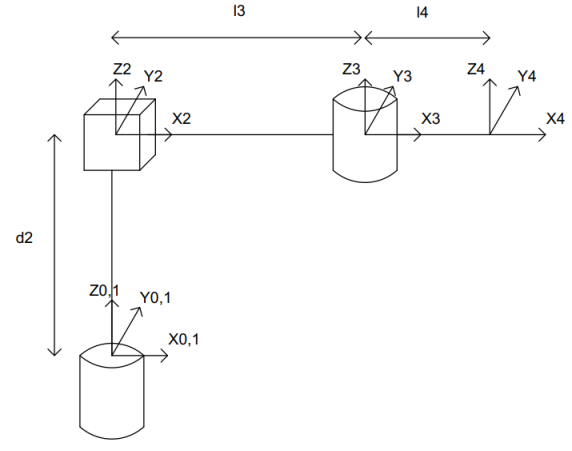
\includegraphics[width=0.7\textwidth]{pictures/set_frame.png} 
        \caption{Setting coordinate frames for robot}
    \end{figure}


    

        
        
    \subsubsection*{Khung xe (mô hình con lắc)}
        \hspace*{0.6cm}Cấu hình robot có thể được mô hình như một con lắc ngược
            \begin{figure}[H]
                \centering
                % \includegraphics[width=0.5\textwidth]{pictures/inverted_pendulum.png} 
                \caption{Sơ đồ tự do của con lắc ngược}
            \end{figure}
            
            Động năng quay của khung xe
            \begin{align}
                K_{p1} = \dfrac{1}{2} I_p \dot{\theta}^2 
            \end{align}
            
            Động năng tịnh tiến của khung xe
            \begin{align}
                K_{p2} = \dfrac{1}{2} M_p v_c^2
            \end{align}
            
            Chọn gốc tọa độ tại ví trí tâm bánh xe, tọa độ khối tâm của con lắc là

            \begin{align}
                (x_c, y_c) = (x+\ell \sin(\theta), \ell \cos \theta) 
            \end{align}
            
            Vận tốc khối tâm của khung xe
            \begin{align}
                (V_{cx}, v_{cy}) = (\dot{x}+\ell \dot{\theta} \cos(\theta), -\ell \dot{\theta}\sin \theta) 
            \end{align}

            Động năng tịnh tiến của khung xe
            \begin{align}
                K_{p2} &= \dfrac{1}{2} M_p \left[(\dot{x}+\ell \dot{\theta} \cos(\theta))^2 + (-\ell \dot{\theta}\sin \theta)^2\right] \nonumber\\
                       &=\dfrac{1}{2} M_p \left[\dot{x}^2 + 2 \ell \dot{x} \dot{\theta} \cos \theta + \ell^2 \dot{\theta}^2\right] 
            \end{align}
            
            Tổng động năng của khung xe
            
            \begin{align}
                K_{p} = K_{p1} + K_{p2} = \dfrac{1}{2} I_p \dot{\theta}^2 + \dfrac{1}{2} M_p \left[\dot{x}^2 + 2 \ell \dot{x} \dot{\theta} \cos \theta + \ell^2 \dot{\theta}^2\right]
            \end{align}

            Do đó tổng động năng của hệ là
            \begin{align}
                K = K_w + K_p &= M_w \dot{x}^2 + \dfrac{I_w}{r^2} \dot{x}^2 + \dfrac{1}{2} I_p \dot{\theta}^2 + \dfrac{1}{2} M_p \left[\dot{x}^2 + 2 \ell \dot{x} \dot{\theta} \cos \theta + \ell^2 \dot{\theta}^2\right] \nonumber\\
                    &= \dfrac{1}{2} \left(2M_w + 2 \dfrac{I_w}{r^2} + M_p\right) \dot{x}^2 + \dfrac{1}{2} \left(M_p \ell^2 + I_p\right)\dot{\theta}^2 + M_p \ell \dot{x} \dot{\theta} \cos \theta \nonumber\\
                    &= \dfrac{1}{2} M_{\Sigma} \dot{x}^2 + \dfrac{1}{2} J \dot{\theta}^2 + M_p \ell \dot{x} \dot{\theta} \cos \theta
             \end{align}
             Với
             \begin{align}
                M_{\Sigma} &= 2M_w + 2 \dfrac{I_w}{r^2} + M_p \nonumber\\
                J &= M_p \ell^2 + I_p \nonumber
             \end{align}
    \subsection*{Thế năng}
            Thế năng của hệ khi khung xe nghiêng một góc $\theta_p$ so với phương thẳng đứng là:
            \begin{align}
                V = M_p g \ell \cos \theta
            \end{align}         


    \subsection*{Phương trình Lagrange}
            Phương trình Lagrange tổng quát cho cơ hệ
            \begin{align}
                \frac{d}{dt} \left( \frac{\partial L}{\partial \dot{q_i}} \right) - \frac{\partial L}{\partial q_i} = Q_i
            \end{align}

            Trong đó
            \begin{itemize}
                \item $L = K - V$: hàm Lagrange
                \item $q_i$: tọa độ suy rộng, trong phạm vi bài báo cáo ta có $q = [x \,\, \theta]^T$
                \item $\dot{q_i}$: đạo hàm theo thời gian của $q_i$
                \item $Q_i$: moment hoặc lực tổng quát (nếu có). Trong phạm vi bài báo cáo ta có $Q_i = [F_x \,\, \tau_\theta]$.
            \end{itemize}

            Hàm Lagrange
            \begin{align}
                L = K - V = \dfrac{1}{2} M_{\Sigma} \dot{x}^2 + \dfrac{1}{2} J \dot{\theta}^2 + M_p \ell \dot{x} \dot{\theta} \cos \theta - M_p g \ell \cos \theta 
            \end{align}    

            Đối với tọa độ suy rộng $x$:
            \begin{align*}
                &\frac{\partial L}{\partial \dot{x}} = M_{\Sigma} \dot{x} + M_p \ell \dot{\theta} \cos \theta\\
                &\frac{d}{dt} \left( \frac{\partial L}{\partial \dot{x}} \right) = M_{\Sigma} \ddot{x} + M_p \ell \ddot{\theta} \cos \theta - M_p \ell \dot{\theta}^2 \sin \theta\\
                &\frac{\partial L}{\partial x} = 0
            \end{align*}

            Do đó
            \begin{align}
                M_{\Sigma} \ddot{x} + M_p \ell \ddot{\theta} \cos \theta - M_p \ell \dot{\theta}^2 \sin \theta = F_x
            \end{align}


            Đối với tọa độ suy rộng $\theta$:
            \begin{align*}
                &\frac{\partial L}{\partial \dot{\theta}} = J \dot{\theta} + M_p \ell \dot{x} \cos \theta\\
                &\frac{d}{dt} \left( \frac{\partial L}{\partial \dot{\theta}} \right) = J \ddot{\theta} + M_p \ell \ddot{x} \cos \theta - M_p \ell \dot{x} \dot{\theta} \sin \theta\\
                &\frac{\partial L}{\partial \theta} = -M_p \ell \dot{x} \dot{\theta} \sin \theta - M_p g \ell (-\sin \theta) = -M_p \ell \dot{x} \dot{\theta} \sin \theta + M_p g \ell \sin \theta
            \end{align*}

            Do đó
            \begin{align}
                J \ddot{\theta} + M_p \ell \ddot{x} \cos \theta - M_p \ell \dot{x} \dot{\theta} \sin \theta + M_p \ell \dot{x} \dot{\theta} \sin \theta - M_p g \ell \sin \theta = \tau_\theta \nonumber\\
                \Leftrightarrow J \ddot{\theta} + M_p \ell \ddot{x} \cos \theta - M_p g \ell \sin \theta = \tau_\theta
            \end{align}

            Từ phương trình (1.13) và (1.15) ta có hệ 

            \begin{equation}
                \begin{cases}
                    M_{\Sigma} \ddot{x} + M_p \ell \ddot{\theta} \cos \theta - M_p \ell \dot{\theta}^2 \sin \theta = F_x \\
                    J \ddot{\theta} + M_p \ell \ddot{x} \cos \theta - M_p g \ell \sin \theta = \tau_\theta
                \end{cases}
            \end{equation}

            Ta đưa về dạng tổng quát
            \begin{equation}
                M(q) \ddot{q} + C (q, \dot{q}) \dot{q} + G(q) = \tau
            \end{equation}
            Trong đó
            \begin{itemize}
                \item $q = [x \,\, \theta]^T$: vector trạng thái
                \item $M(q)$: ma trận quán tính
                \item $C(q, \dot{q})$: ma trận Coriolis và ly tâm
                \item $G(q)$: vector trọng lực
                \item $\tau$: moment xoắn điều khiển từ động cơ
            \end{itemize} 
            Ta được
            \begin{align*}
                &\underbrace{
                \begin{bmatrix}
                M_\Sigma & M_p \ell \cos \theta\\
                M_p \ell  \cos \theta & J
                \end{bmatrix}
                }_{M(q)}
                \begin{bmatrix}
                \ddot{x} \\ \ddot{\theta}
                \end{bmatrix}
                +
                \underbrace{
                \begin{bmatrix}
                0 & -M_p \ell \dot{\theta} \sin \theta \\
                0 & 0
                \end{bmatrix}
                }_{C(q, \dot{q})}
                \begin{bmatrix}
                \dot{x} \\ \dot{\theta}
                \end{bmatrix} 
                +
                \underbrace{
                \begin{bmatrix}
                0 \\
                -M_p g \ell \sin \theta
                \end{bmatrix}
                }_{G(q)}
                =
                \underbrace{
                \begin{bmatrix}
                F_x \\
                \tau
                \end{bmatrix}
                }
            \end{align*}
        
        Trong chương tiếp theo, ta sẽ tiến hành thiết kế và mô phỏng các bộ điều khiển dựa trên hàm truyền đã thu được.
            
        
       
    
\chapter{DETERMINING D-H PARAMETERS}

\section{Topic}
Determine the Denavit-Hartenberg parameters for the robot model.

\section{Theory}
The Denavit-Hartenberg notation is introduced as a systematic method of describing the kinematic relationship ${}^{i-1}T_i$ using only four parameters \cite{1}:

\begin{center}
     \begin{tabular}{|c|l|l|}
          \hline
          $\alpha$ & Link twist & Describe the link itself \\
          \hline
          $a$ & Link length & \\
          \hline
          $d$ & Link offset & Describe the link's connection to neighboring link \\
          \hline
          $\theta$ & Joint angle & \\
          \hline
          \multicolumn{3}{|l|}{If the joint is:} \\
          \hline
          \multicolumn{2}{|l|}{Revolute: $\theta$ joint variable} & The other three are fixed link parameters \\
          \hline
          \multicolumn{2}{|l|}{Prismatic: $d$ joint variable} & \\
          \hline
          \end{tabular}
\end{center}



\section{Application}
We got the D-H table:

\begin{center}
\begin{tabular}{|c|c|c|c|c|}
\hline
$i$ & $a_i$ & $\alpha_i$ & $d_i$ & $\theta_i$ \\
\hline
1 & 0 & 0 & 0 & $\theta_1$ \\
2 & 0 & 0 & $d_2$ & 0 \\
3 & $\ell_3$ & 0 & 0 & 0 \\
4 & $\ell_4$ & 0 & 0 & $\theta_4$ \\
\hline
\end{tabular}
\end{center}


Limitations of the D-H notation:
\begin{align*}
     &\ell_3 = 1000 \,\mathrm{mm}\\
     &\ell_4 = 300 \,\mathrm{mm}\\
     &d_2 \in [2150; 2750] \\
     &\theta_1 \in [0^\circ; 360^\circ] \\
     &\theta_4 \in [-90^\circ; 90^\circ]
\end{align*}


    \chapter{KINEMATIC PROBLEM}

\section{Topic}
Formulate the forward kinematic problem. Then determine the coordinates of the end-point 
according to the three joint variables. Make a plot for a certain case.
 
\section{Theory}

The transformaytion matrix $^{i-1}_{i}T$ to transform coordinate frames \textbf{$B_i$} to \textbf{$B_i - 1$} is represented as a product of four basic transformations using paramaters of link $(i)$ and joint $i$

\begin{align}
^{i-1}_{i}T = 
\begin{bmatrix}
\cos(\theta_i) & -\sin(\theta_i)\cos(\alpha_i) & \sin(\theta_i)\sin(\alpha_i) & a_i\cos(\theta_i) \\
\sin(\theta_i) & \cos(\theta_i)\cos(\alpha_i) & -\cos(\theta_i)\sin(\alpha_i) & a_i\sin(\theta_i) \\
0 & \sin(\alpha_i) & \cos(\alpha_i) & d_i \\
0 & 0 & 0 & 1
\end{bmatrix}
\end{align}

To find the single transformation that relates frame \{$i$\} to frame \{0\}, the transformation matrices of every link are then multiplied together:

\begin{equation}
^{0}_{i}T = ^{0}_{1}T \ ^{1}_{2}T\ ... \ ^{i-1}_{i}T
\end{equation}

This transformation $^{0}_{i}T$ is a function of all $i$ joint variables. If the robot's joint-position sensors are queried, the Cartesian position and orientation of the end effector could be computed by $^{0}_{i}T$.



\section{Application}
We have:

\begin{equation}
    ^{0}T_{1} = 
    \begin{bmatrix}
    \cos\theta_1 & -\sin\theta_1 & 0 & 0 \\
    \sin\theta_1 & \cos\theta_1 & 0 & 0 \\
    0 & 0 & 1 & 0 \\
    0 & 0 & 0 & 1
    \end{bmatrix}
\end{equation}

\begin{equation}
    ^{1}T_{2} = 
    \begin{bmatrix}
    1 & 0 & 0 & 0 \\
    0 & 1 & 0 & 0 \\
    0 & 0 & 1 & d_2 \\
    0 & 0 & 0 & 1
    \end{bmatrix}
\end{equation}

\begin{equation}
    ^{2}T_{3} = 
    \begin{bmatrix}
    1 & 0 & 0 & \ell_3 \\
    0 & 1 & 0 & 0 \\
    0 & 0 & 1 & 0 \\
    0 & 0 & 0 & 1
    \end{bmatrix}
\end{equation}

\begin{equation}
    ^{3}T_{4} = 
    \begin{bmatrix}
    \cos\theta_4 & -\sin\theta_4 & 0 & \ell_4\cdot\cos\theta_4 \\
    \sin\theta_4 & \cos\theta_4 & 0 & \ell_4\cdot\sin\theta_4 \\
    0 & 0 & 1 & 0 \\
    0 & 0 & 0 & 1
    \end{bmatrix}
\end{equation}

Thus

\begin{equation*}
    ^{0}T_{4} = ^{0}T_{1}.^{1}T_{2}.^{2}T_{3}.^{3}T_{4}
    = 
    \begin{bmatrix}
    \cos(\theta_1 + \theta_4) & -\sin(\theta_1 + \theta_4) & 0 & \ell_4.\cos(\theta_1 + \theta_4) + \ell_3.\cos\theta_1 \\
    \sin(\theta_1 + \theta_4) & \cos(\theta_1 + \theta_4) & 0 & \ell_4.\sin(\theta_1 + \theta_4) + \ell_3.\sin\theta_1 \\
    0 & 0 & 1 & d_2 \\
    0 & 0 & 0 & 1
    \end{bmatrix}
\end{equation*}

In conclusion, we have the solution for the forward kinematic problem as below


\begin{equation}
    \begin{bmatrix}
        x  \\
        y \\
        z 
        \end{bmatrix}
    = 
    \begin{bmatrix}
        \ell_4.\cos(\theta_1 + \theta_4) + \ell_3.\cos\theta_1 \\
        \ell_4.\sin(\theta_1 + \theta_4) + \ell_3.\sin\theta_1 \\
        d_2 
        \end{bmatrix}
\end{equation}

Make a plot for a certain case: \\
\hspace*{0.6cm} During the time \( t \) from 0s to 10s, the input \( (\theta_1, d_2, \theta_4) \) gradually increases from \( (0^\circ, 2200, 0^\circ) \) to \( (90^\circ, 2700, 90^\circ) \). Using MATLAB, the position \( (x, y, z \) of the end-effector can be plotted as below:
\begin{figure}[H]
    \centering
    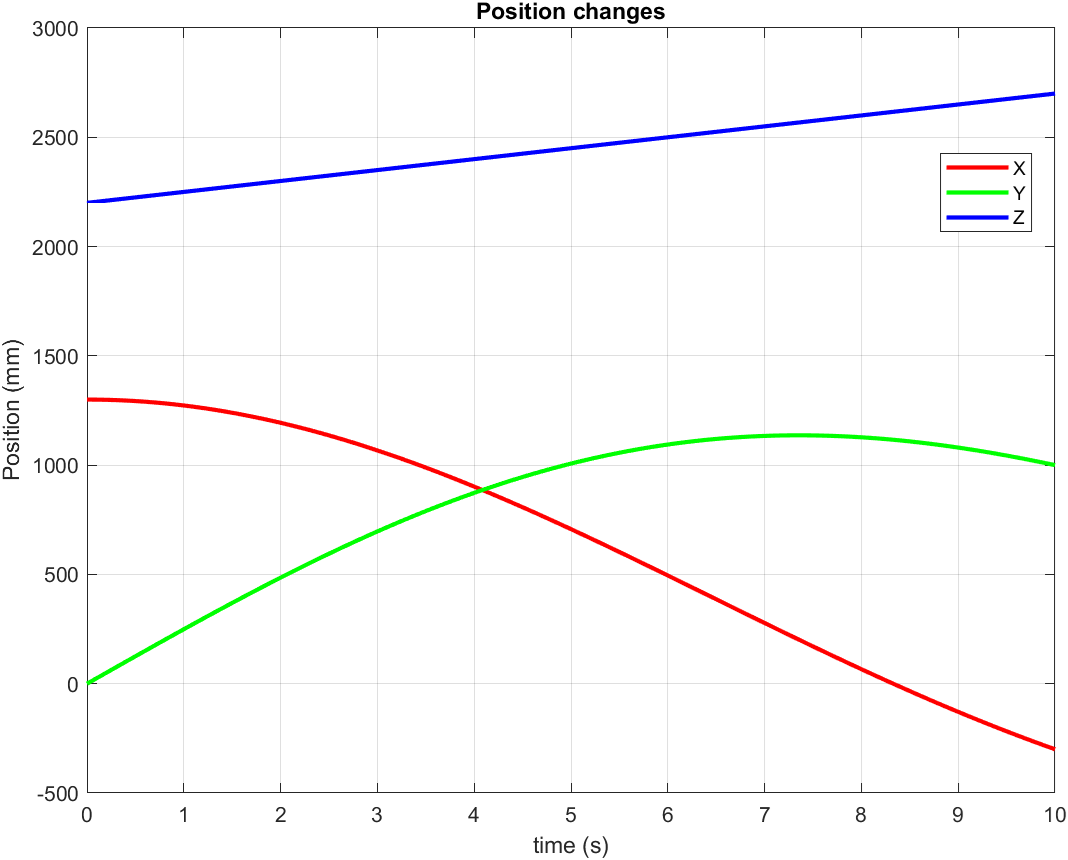
\includegraphics[width=0.8\textwidth]{pictures/test_forward.png}
    \caption{The position of the end-effector $(x,y,z)$ with respect to time}
    \label{fig:forward_kinematic}
\end{figure}
Solution check:
\begin{itemize}
    \item At time \( t = 0 \) s, the end-effector is at position \( (x,y,z) = (1300,0,2200) \) mm. Correct!\\
    \item At time \( t = 10 \) s, the end-effector is at position \( (x,y,z) = (-300,1000,2700) \) mm. Correct!\\
\end{itemize}
So we can confirm the accurate of the solution.
% check the forward kinematic problem with the following values:
    \chapter{INVERSE KINEMATIC PROBLEM}
    \section{Topic}
        Formulate the inverse kinematic problem. Then determine the three joint values according 
        to the coordinates of the end-point. Make a plot for a certain case.
    \section{Theory}
        Inverse kinematics is the mathematical process of calculating the variable joint parameters 
        needed to place the end of a kinematic chain which is, in this project, the position of the end 
        effector of a robot arm [1].

    \section{Application}

        We have the forward kinematic equation:
        \begin{equation*}
            \begin{bmatrix}
                x  \\
                y \\
                z 
                \end{bmatrix}
            = 
            \begin{bmatrix}
                \ell_4.\cos(\theta_1 + \theta_4) + \ell_3.\cos\theta_1 \\
                \ell_4.\sin(\theta_1 + \theta_4) + \ell_3.\sin\theta_1 \\
                d_2 
                \end{bmatrix}
        \end{equation*}
        The position of the end-effector (X,Y,Z) can be extracted from the matrix as below:
    \begin{align}
        &x = \ell_4.\cos(\theta_1 + \theta_4) + \ell_3.\cos\theta_1\\
        &y = \ell_4.\sin(\theta_1 + \theta_4) + \ell_3.\sin\theta_1\\
        &z = d_2 \\
    \end{align}
    From (2.1) and (2.2) we have
    \begin{align*}
        x^2 + y^2 &= \ell_4^2 + \ell_3^2 + 2 \ell_3 \cdot \ell_4 \left[ \cos(\theta_1 + \theta_4) \cdot \cos \theta_1 + \sin(\theta_1 + \theta_4) \cdot \sin \theta_1 \right] \\
        &= \ell_4^2 + \ell_3^2 + 2 \ell_3 \cdot \ell_4 \cos(\theta_1 + \theta_4 - \theta_1) \\
        &= \ell_4^2 + \ell_3^2 + 2 \ell_3 \cdot \ell_4 \cos(\theta_4) \\
    \end{align*}
    Set
    \begin{equation*}
        a = \cos(\theta_4) = \frac{x^2 + y^2 - \ell_4^2 - \ell_3^2}{2 \ell_3 \cdot \ell_4}
    \end{equation*}
    Thus
    \begin{equation*}
        \theta_4 = \operatorname{atan2}\left( \pm \sqrt{1 - a^2}, a \right)
    \end{equation*}
    The x and y components can be expressed as:
    \begin{align*}
        x \cos \theta_1 + y \sin \theta_1 &= \ell_4 \cdot \cos(\theta_1 + \theta_4) \cos \theta_1 + \ell_4 \cdot \sin(\theta_1 + \theta_4) \cdot \sin \theta_1 + \ell_3 \\
        &= \ell_4 \cdot \cos(\theta_4) + \ell_3 \\
    \end{align*}
    We can rewrite
    \begin{equation*}
        x \cos \theta_1 + y \sin \theta_1 = \sqrt{x^2 + y^2} \left( \frac{x}{\sqrt{x^2 + y^2}} \cos \theta_1 + \frac{y}{\sqrt{x^2 + y^2}} \sin \theta_1 \right) \\
    \end{equation*}
    Set
    \begin{align*} 
        \cos \phi &= \frac{x}{\sqrt{x^2 + y^2}} \\
        \sin \phi &= \frac{y}{\sqrt{x^2 + y^2}} \\
        \phi &= \operatorname{atan2}(y, x) 
    \end{align*}
    Thus we have
    \begin{align*}
        \sqrt{x^2 + y^2} \left( \cos \phi \cdot \cos \theta_1 + \sin \phi \cdot \sin \theta_1 \right) &= \ell_4 \cdot \cos(\theta_4) + \ell_3 \\
    \end{align*}
    Infer the following:
    \begin{align*}
        \cos(\theta_1 - \phi) &= \frac{\ell_4 \cdot a + \ell_3}{\sqrt{x^2 + y^2}} \\
        \sin(\theta_1 - \phi) &= \pm \frac{\sqrt{x^2 + y^2 - \left( \ell_4 \cdot a + \ell_3 \right)^2}}{\sqrt{x^2 + y^2}} \\
        \Rightarrow  \theta_1 - \phi &= \operatorname{atan2}\left( \pm \sqrt{x^2 + y^2 - \left( \ell_4 \cdot a + \ell_3 \right)^2}, \ell_4 \cdot a + \ell_3 \right) \\
        \Rightarrow  \theta_1 &= \phi + \operatorname{atan2}\left( \pm \sqrt{x^2 + y^2 - \left( \ell_4 \cdot a + \ell_3 \right)^2}, \ell_4 \cdot a + \ell_3 \right) \\
        &= \operatorname{atan2}(y, x) + \operatorname{atan2}\left( \pm \sqrt{x^2 + y^2 - \left( \ell_4 \cdot \cos(\theta_4) + \ell_3 \right)^2}, \ell_4 \cdot \cos(\theta_4) + \ell_3 \right) \\
    \end{align*}
    Conclusion, we have the following solution for the inverse kinematic problem:
    \begin{align*}
        &\begin{cases}
        \theta_1 = \operatorname{atan2}(y, x) + \operatorname{atan2}\left( \pm \sqrt{x^2 + y^2 - \left( \ell_4 \cdot \cos(\theta_4) + \ell_3 \right)^2}, \ell_4 \cdot \cos(\theta_4) + \ell_3 \right) \\
        d_2 = z \\
        \theta_4 = \operatorname{atan2}\left(\pm \sqrt{1 - a^2}, a \right)
        \end{cases} \\
    \end{align*}
    or can rewrite as:
    \begin{equation*}
        \begin{bmatrix}
            \theta_1  \\
            d_2 \\
            \theta_4 
            \end{bmatrix}
        = 
        \begin{bmatrix}
            \operatorname{atan2}(y, x) + \operatorname{atan2}\left( \pm \sqrt{x^2 + y^2 - \left( \ell_4 \cdot \cos(\theta_4) + \ell_3 \right)^2}, \ell_4 \cdot \cos(\theta_4) + \ell_3 \right) \\
            Z \\
            \operatorname{atan2}\left(\pm \sqrt{1 - a^2}, a \right) \\
            \end{bmatrix}
    \end{equation*}
    with
    \begin{equation*}
        a = \frac{x^2 + y^2 - \ell_4^2 - \ell_3^2}{2 \ell_3 \cdot \ell_4}
    \end{equation*}

Solution check:\\

    As forward kinematic solution, with the input \( (\theta_1, d_2, \theta_4) = (0^\circ, 2200, 0^\circ) \), the position of the end-effector is \( (x, y, z) = (1300, 0, 2200) \).

    Using \( (x, y, z) = (1300, 0, 2200) \) as an input to inverse function, we got \( (\theta_1, d_2, \theta_4)  = (0^\circ, 2200, 0^\circ) \).
    
    Similarly, using \( (x,y,z) = (-300,1000,2700) \) as an input to inverse function, we got \( (\theta_1, d_2, \theta_4) = (90^\circ,2700, 90^\circ) \). Correct.
    
    So we can confirm the accurate of the solution.
    \chapter{WORKSPACE}
\section{Topic}
Give a comment on the workspace.
\section{Theory}
Existing of any solution raises the question of the manipulator's workspace, which is the volume of space that the end-effector of the manipulator can reach.
\section{Application}
We have: 
\[
\left\{
\begin{aligned}
x &= \ell_4 \cdot \cos(\theta_1 + \theta_4) + \ell_3 \cdot \cos\theta_1 \\
y &= \ell_4 \cdot \sin(\theta_1 + \theta_4) + \ell_3 \cdot \sin\theta_1 \\
z &= d_2
\end{aligned}
\right.
\]
With:
\begin{itemize}
    \item $\ell_3 = 1000\,\text{mm}$
    \item $\ell_4 = 300\,\text{mm}$
    \item $d_2 \in [2150; 2750]$
    \item $\theta_1 \in [0^\circ; 360^\circ]$
    \item $\theta_4 \in [-90^\circ; 90^\circ]$
\end{itemize}
Next:
\[
    x^2 + y^2 = \ell_4^2 + \ell_3^2 + 2\ell_3 \ell_4 \cos(\theta_4)
\]
\[
    \Leftrightarrow \cos(\theta_4) = \frac{x^2 + y^2 - \ell_4^2 - \ell_3^2}{2 \ell_3 \ell_4}
\]
We also have:
\[
    0 \leq \cos(\theta_4) \leq 1
\]
\[
    \Rightarrow 0 \leq x^2 + y^2 \leq (\ell_4 + \ell_3)^2
\]
\[
\Rightarrow 
\left\{
\begin{aligned}
0 &\leq x^2 + y^2 \leq 1690000 \\
d_2 &\in [2150; 2750] \\
\theta_1 &\in [0^\circ; 360^\circ] \\
\theta_4 &\in [-90^\circ; 90^\circ]
\end{aligned}
\right.
\]
To simplify matters, we remove the mechanical constraint, the joints can be fully rotated. Therefore, our workspace is idealized.
\begin{figure}[H]
    \centering
    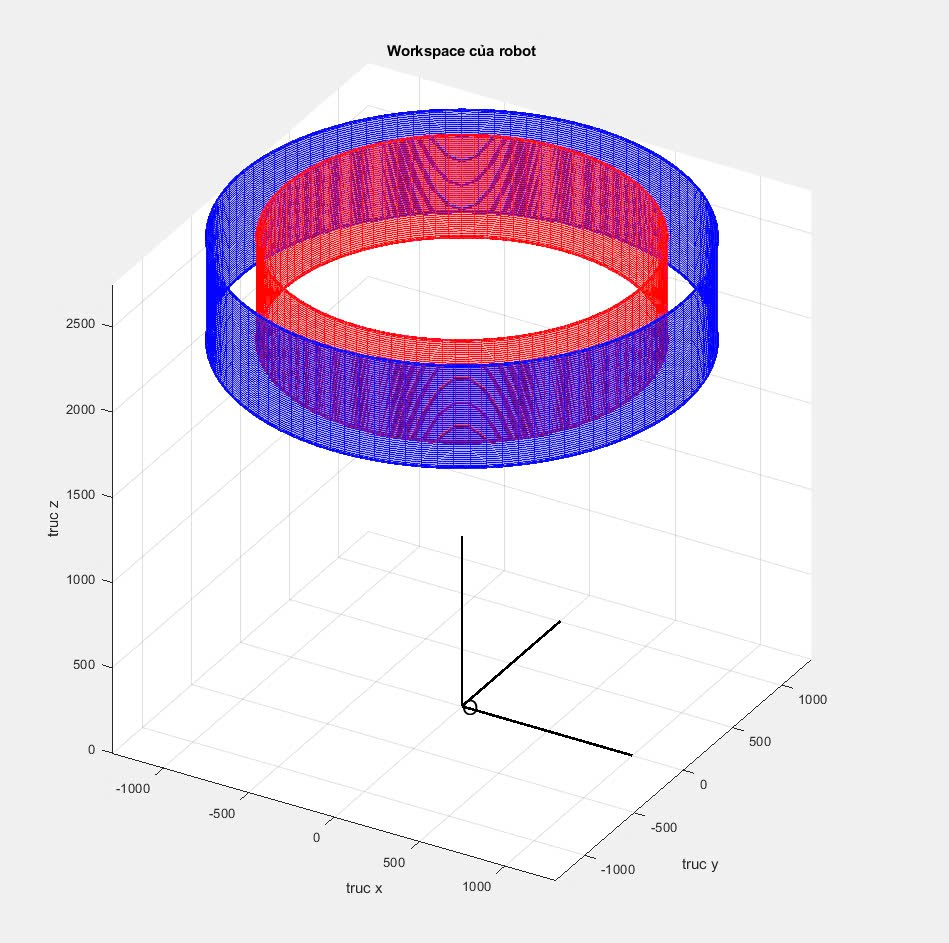
\includegraphics[width=0.5\textwidth]{pictures/workspace1.png} 
    \caption{Workspace of the robot}
\end{figure}
\begin{figure}[H]
    \centering
    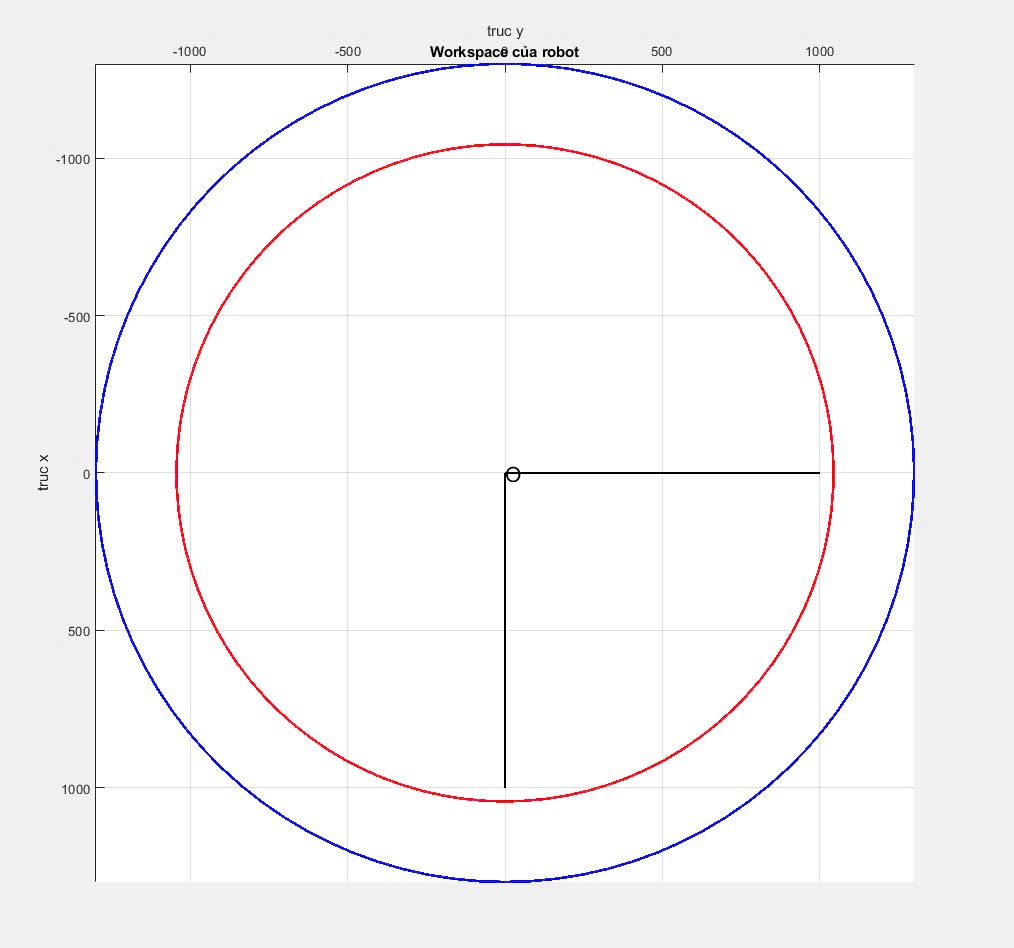
\includegraphics[width=0.5\textwidth]{pictures/workspace2.png} 
    \caption{Workspace of the robot another view}
\end{figure}
\chapter{JACOBIAN MATRIX}
\section{Topic}
Formulate the Jacobian matrix for this robot. Is there any singularity?
\section{Theory}
The Jacobian is a multidimensional form of the derivative. The 6 x 6 matrix of partial derivatives is the Jacobian $J$, as mapping velocities in $X$ to those in $Y$. \\
In the field of robotics, Jacobians are used to relate joint velocities to Cartesian velocities of the tip of the arm.

\[
{}^0\mathbf{V} = {}^0\!J(\theta) \, \dot{\theta}
\]

All manipulators have singularities at:
\begin{itemize}
    \item The boundary of their workspace.
    \item Most have loci of singularities inside their workspace.
\end{itemize}
\section{Application}
Vector of joint variables:
\[
\mathbf{Q} = \begin{bmatrix} \theta_1 & d_2 & \theta_4 \end{bmatrix}^T
\]
Position-orientation state vector $\mathbf{X}$:
\[
\mathbf{X} = \begin{bmatrix} p_x & p_y & d_2 & 0 & 0 & \theta_1 + \theta_4 \end{bmatrix}^T
\]
\[
= \begin{bmatrix} 
\ell_4 \cos(\theta_1 + \theta_4) + \ell_3 \cos \theta_1 & 
\ell_4 \sin(\theta_1 + \theta_4) + \ell_3 \sin \theta_1 & 
d_2 & 
0 & 
0 & 
\theta_1 + \theta_4 
\end{bmatrix}^T
\]
The Jacobian matrix $J$ is the partial derivative of the position vector $\mathbf{X}$ with respect to the joint variable vector $\mathbf{q}$:

\[
J = \frac{\partial \mathbf{X}}{\partial \mathbf{q}} =
\begin{bmatrix}
\frac{\partial p_x}{\partial \theta_1} & \frac{\partial p_x}{\partial d_2} & \frac{\partial p_x}{\partial \theta_4} \\
\frac{\partial p_y}{\partial \theta_1} & \frac{\partial p_y}{\partial d_2} & \frac{\partial p_y}{\partial \theta_4} \\
\frac{\partial d_2}{\partial \theta_1} & \frac{\partial d_2}{\partial d_2} & \frac{\partial d_2}{\partial \theta_4} \\
0 & 0 & 0 \\
0 & 0 & 0 \\
\frac{\partial (\theta_1 + \theta_4)}{\partial \theta_1} & \frac{\partial (\theta_1 + \theta_4)}{\partial d_2} & \frac{\partial (\theta_1 + \theta_4)}{\partial \theta_4}
\end{bmatrix}
\]

\[
=
\begin{bmatrix}
-\ell_4 \sin(\theta_1 + \theta_4) - \ell_3 \sin\theta_1 & 0 & -\ell_4 \sin(\theta_1 + \theta_4) \\
\ell_4 \cos(\theta_1 + \theta_4) + \ell_3 \cos\theta_1 & 0 & \ell_4 \cos(\theta_1 + \theta_4) \\
0 & 1 & 0 \\
0 & 0 & 0 \\
0 & 0 & 0 \\
1 & 0 & 1
\end{bmatrix}
\]
\[
\Rightarrow \text{ Control matrix } \mathbf{J} = 
\begin{bmatrix}
-\ell_4 \sin(\theta_1 + \theta_4) - \ell_3 \sin \theta_1 & 0 & -\ell_4 \sin(\theta_1 + \theta_4) \\
\ell_4 \cos(\theta_1 + \theta_4) + \ell_3 \cos \theta_1 & 0 & \ell_4 \cos(\theta_1 + \theta_4) \\
0 & 1 & 0
\end{bmatrix}
\]
\textbf{Case of Jacobian Singularity}
\[
J = \begin{bmatrix}
-l_4 \sin(\theta_0 + \theta_4) & -l_3 \sin\theta_1 & 0 & -l_4 \sin(\theta_1 + \theta_4) \\
l_4 \cos(\theta_0 + \theta_4) + l_3 \cos\theta_1 & 0 & 0 & l_4 \cos(\theta_1 + \theta_4) \\
0 & 1 & 0 & 0 \\
0 & 0 & 1 & 0
\end{bmatrix}
\]

\[
\det(J_a) = a_{11} \cdot (a_{22} \cdot a_{33} - a_{23} \cdot a_{32}) - a_{12} \cdot (a_{21} \cdot a_{33} - a_{23} \cdot a_{31}) + a_{13} \cdot (a_{21} \cdot a_{32} - a_{22} \cdot a_{31})
\]
\[
= [-l_4 \sin(\theta_0 + \theta_4) - l_3 \sin\theta_1][l_4 \cos(\theta_1 + \theta_4)] + [-l_4 \sin(\theta_1 + \theta_4)][l_4 \cos(\theta_0 + \theta_4) + l_3 \cos\theta_1]
\]
\[
-l_4^2 \sin(\theta_0 + \theta_4) \cos(\theta_1 + \theta_4) + l_3 \sin\theta_1 l_4 \cos(\theta_1 + \theta_4) - l_4^2 \sin(\theta_1 + \theta_4)\cos(\theta_0 + \theta_4) 
\]
\[
- l_3 l_4 \sin(\theta_1 + \theta_4)\cos\theta_1
\]

\[
= l_3 l_4 [\sin\theta_1 \cdot \cos(\theta_1 + \theta_4) - l_4 l_3 \sin(\theta_1 + \theta_4) \cdot \cos\theta_1]
\]

\[
= -l_3 \cdot l_4 \cdot \sin(-\theta_4)
\]

\[
\det(J_a) = 0 \iff -l_4 \cdot l_3 \cdot \sin(-\theta_4) = 0
\]

\[
\iff -l_3 \cdot l_4 \cdot \sin(\theta_4) = 0
\]

\[
\iff \theta_4 = k\pi (k \in \mathbb{Z}); \theta_4 \in [-90^\circ, 90^\circ]
\]

\[
\Rightarrow \text{The point is within the range where } \theta_4 = 0
\]
    \chapter{SIMULATING THE MOTION OF ROBOT}
    \section{Topic}
    Simulate the motion of this robot to plot initial letters from the first names of your team members on a certain plane that is perpendicular to axis \( z_0 \).
    \section{Theory}
        Simulate robot in simscape $(\theta_1, d_2, \theta_4)$ change from $(0,2200, 0)$ to $(90^{\circ}, 2700, 90^{\circ})$.
        \begin{figure}[H]
            \centering
            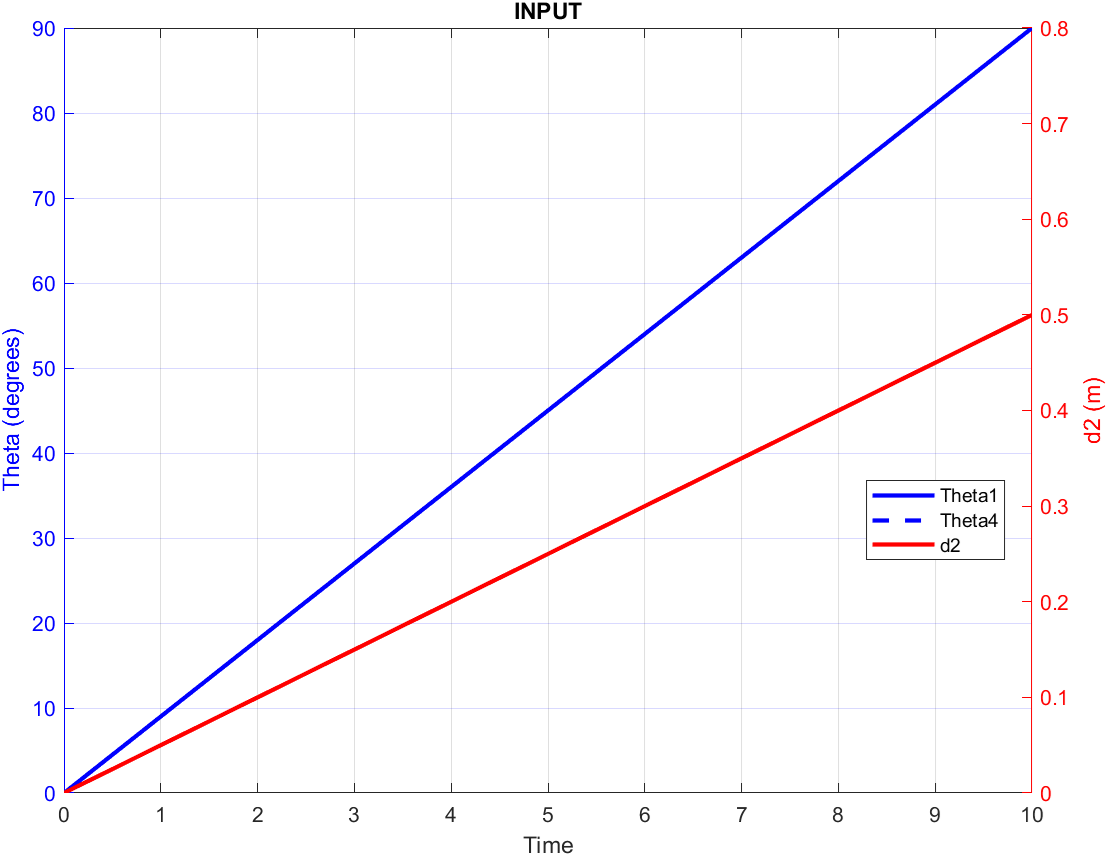
\includegraphics[width=0.8\textwidth]{pictures/theta_d_change.png}
            \caption{Simulation of the robot}
            \label{fig:theta_d_change}
        \end{figure}
        Apply to forward, get position of end-effector \( (x,y,z) \) with respect to time \( t \)
        \begin{figure}[H]
            \centering
            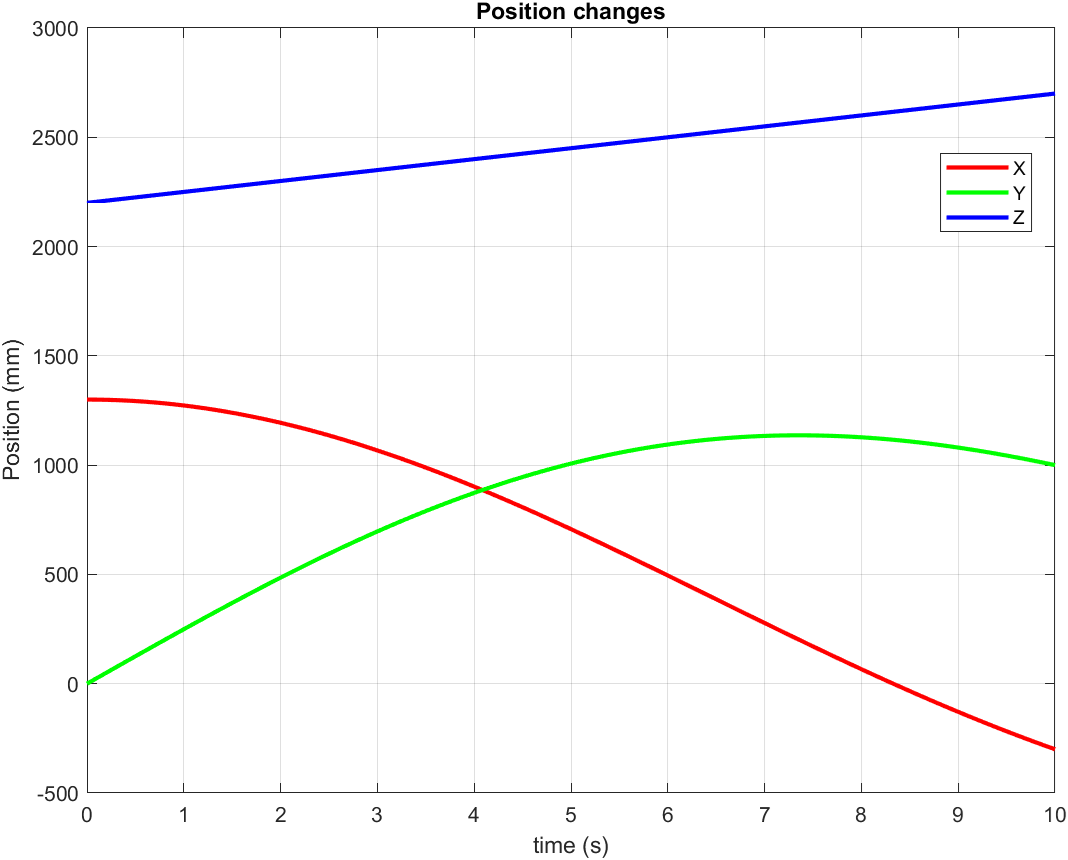
\includegraphics[width=0.8\textwidth]{pictures/test_forward.png}
            \caption{Simulation of the robot}
            \label{fig:test_forward}
        \end{figure}

        
    \section{Application}
    Modeling robot by Solidworks then convert to step file, this is suitable for Simscape 
    Multibody Link.
    \begin{figure}[H]
        \centering
        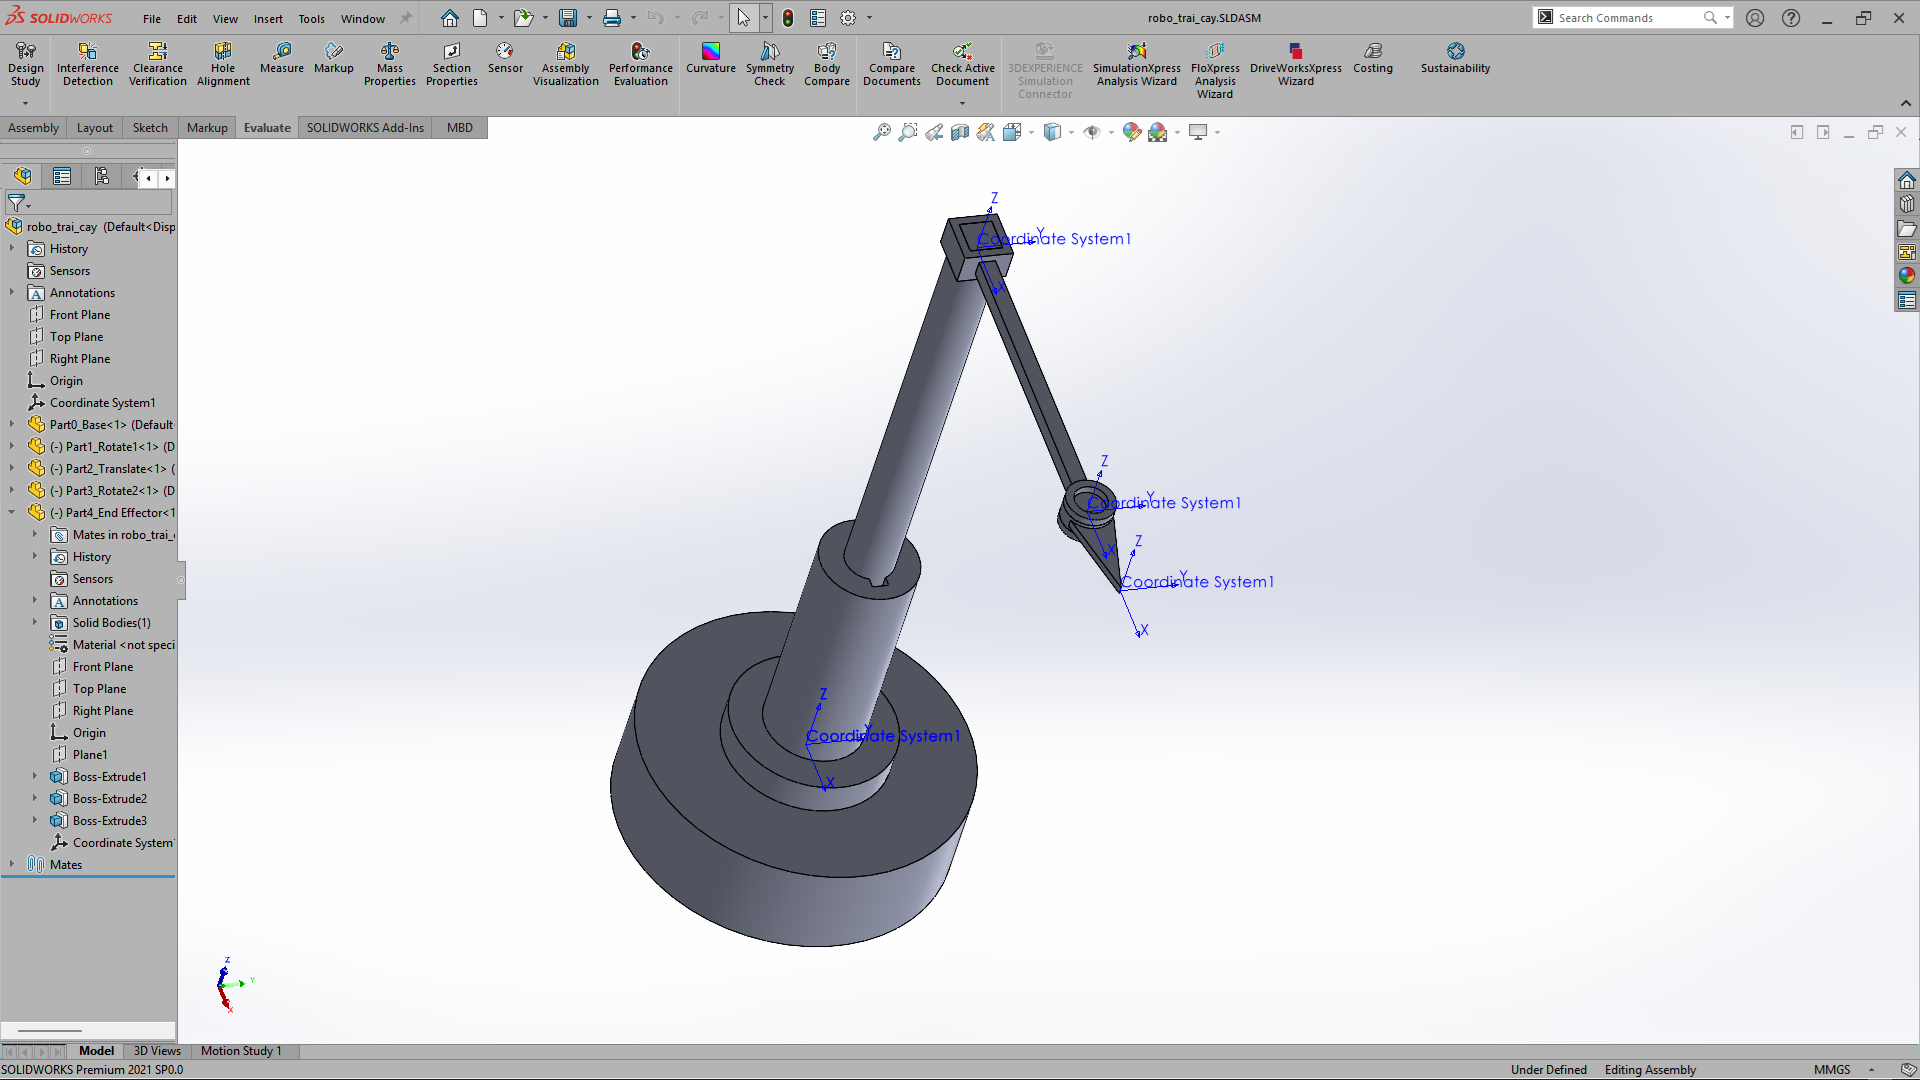
\includegraphics[width=0.8\textwidth]{pictures/solid.png}
        \caption{Robot model in Solidworks}
        \label{fig:robot_model}
    \end{figure}
    Model in Simscape Multibody Link
    \begin{figure}[H]
        \centering
        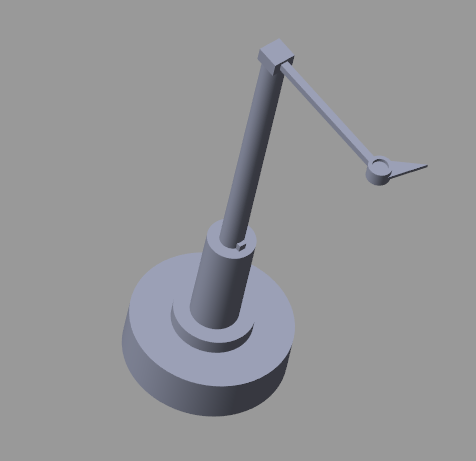
\includegraphics[width=0.6\textwidth]{pictures/simscape.png}
        \caption{Robot model in Simscape Multibody Link}
        \label{fig:simscape_model}
    \end{figure}
    Block diagrams of Matlab Simulink is as the follow:
    \begin{figure}[H]
        \centering
        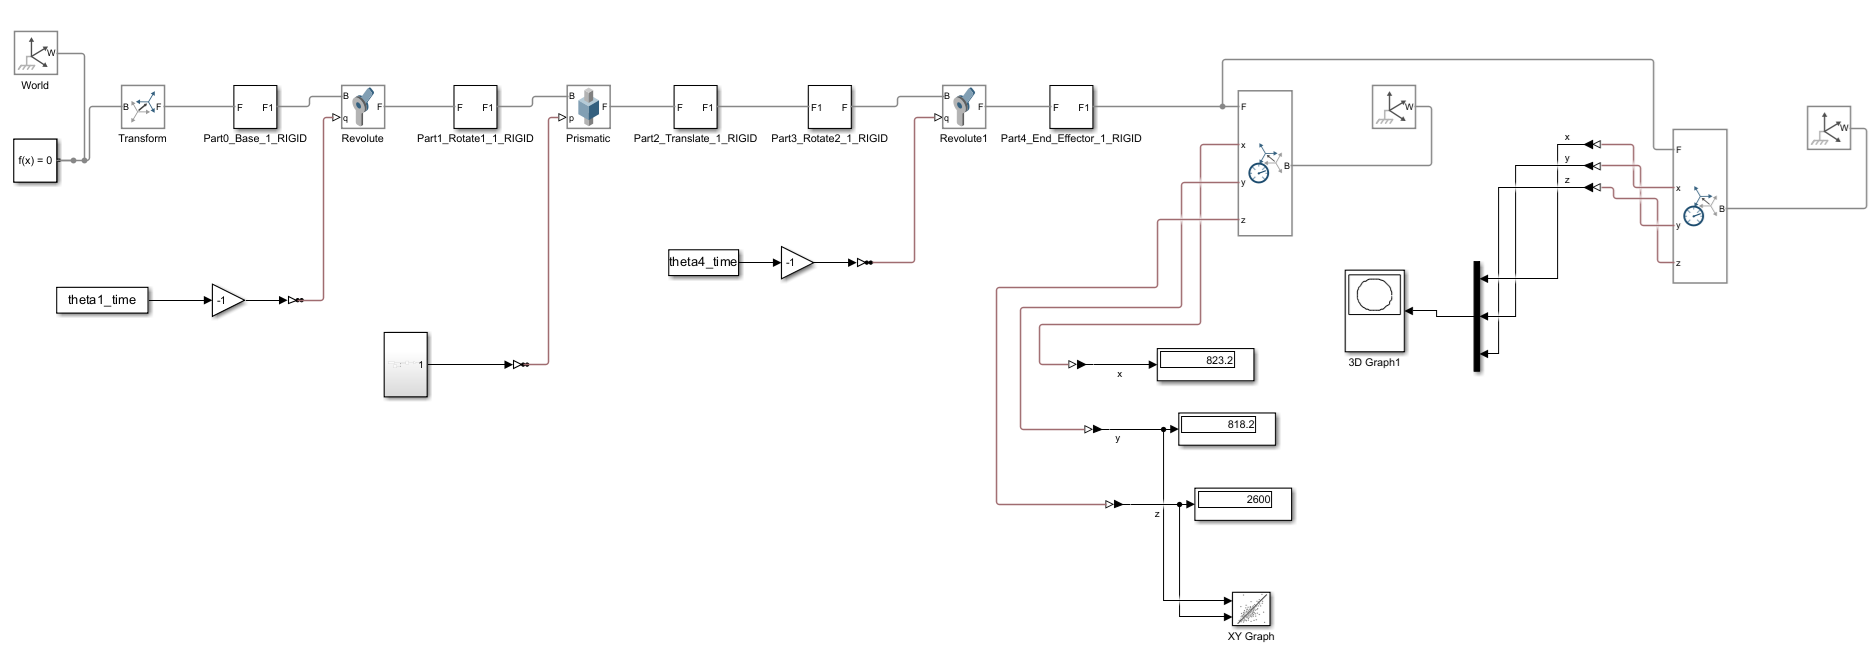
\includegraphics[width=1\textwidth]{pictures/simulink.png}
        \caption{Block diagram of Matlab Simulink}
        \label{fig:simulink_block_diagram}
    \end{figure}
    Results of simulation: \\
    \hspace*{0.6cm}Position \( (x,y,z) \) of robot from transsform sensor
    \begin{figure}[H]
        \centering
        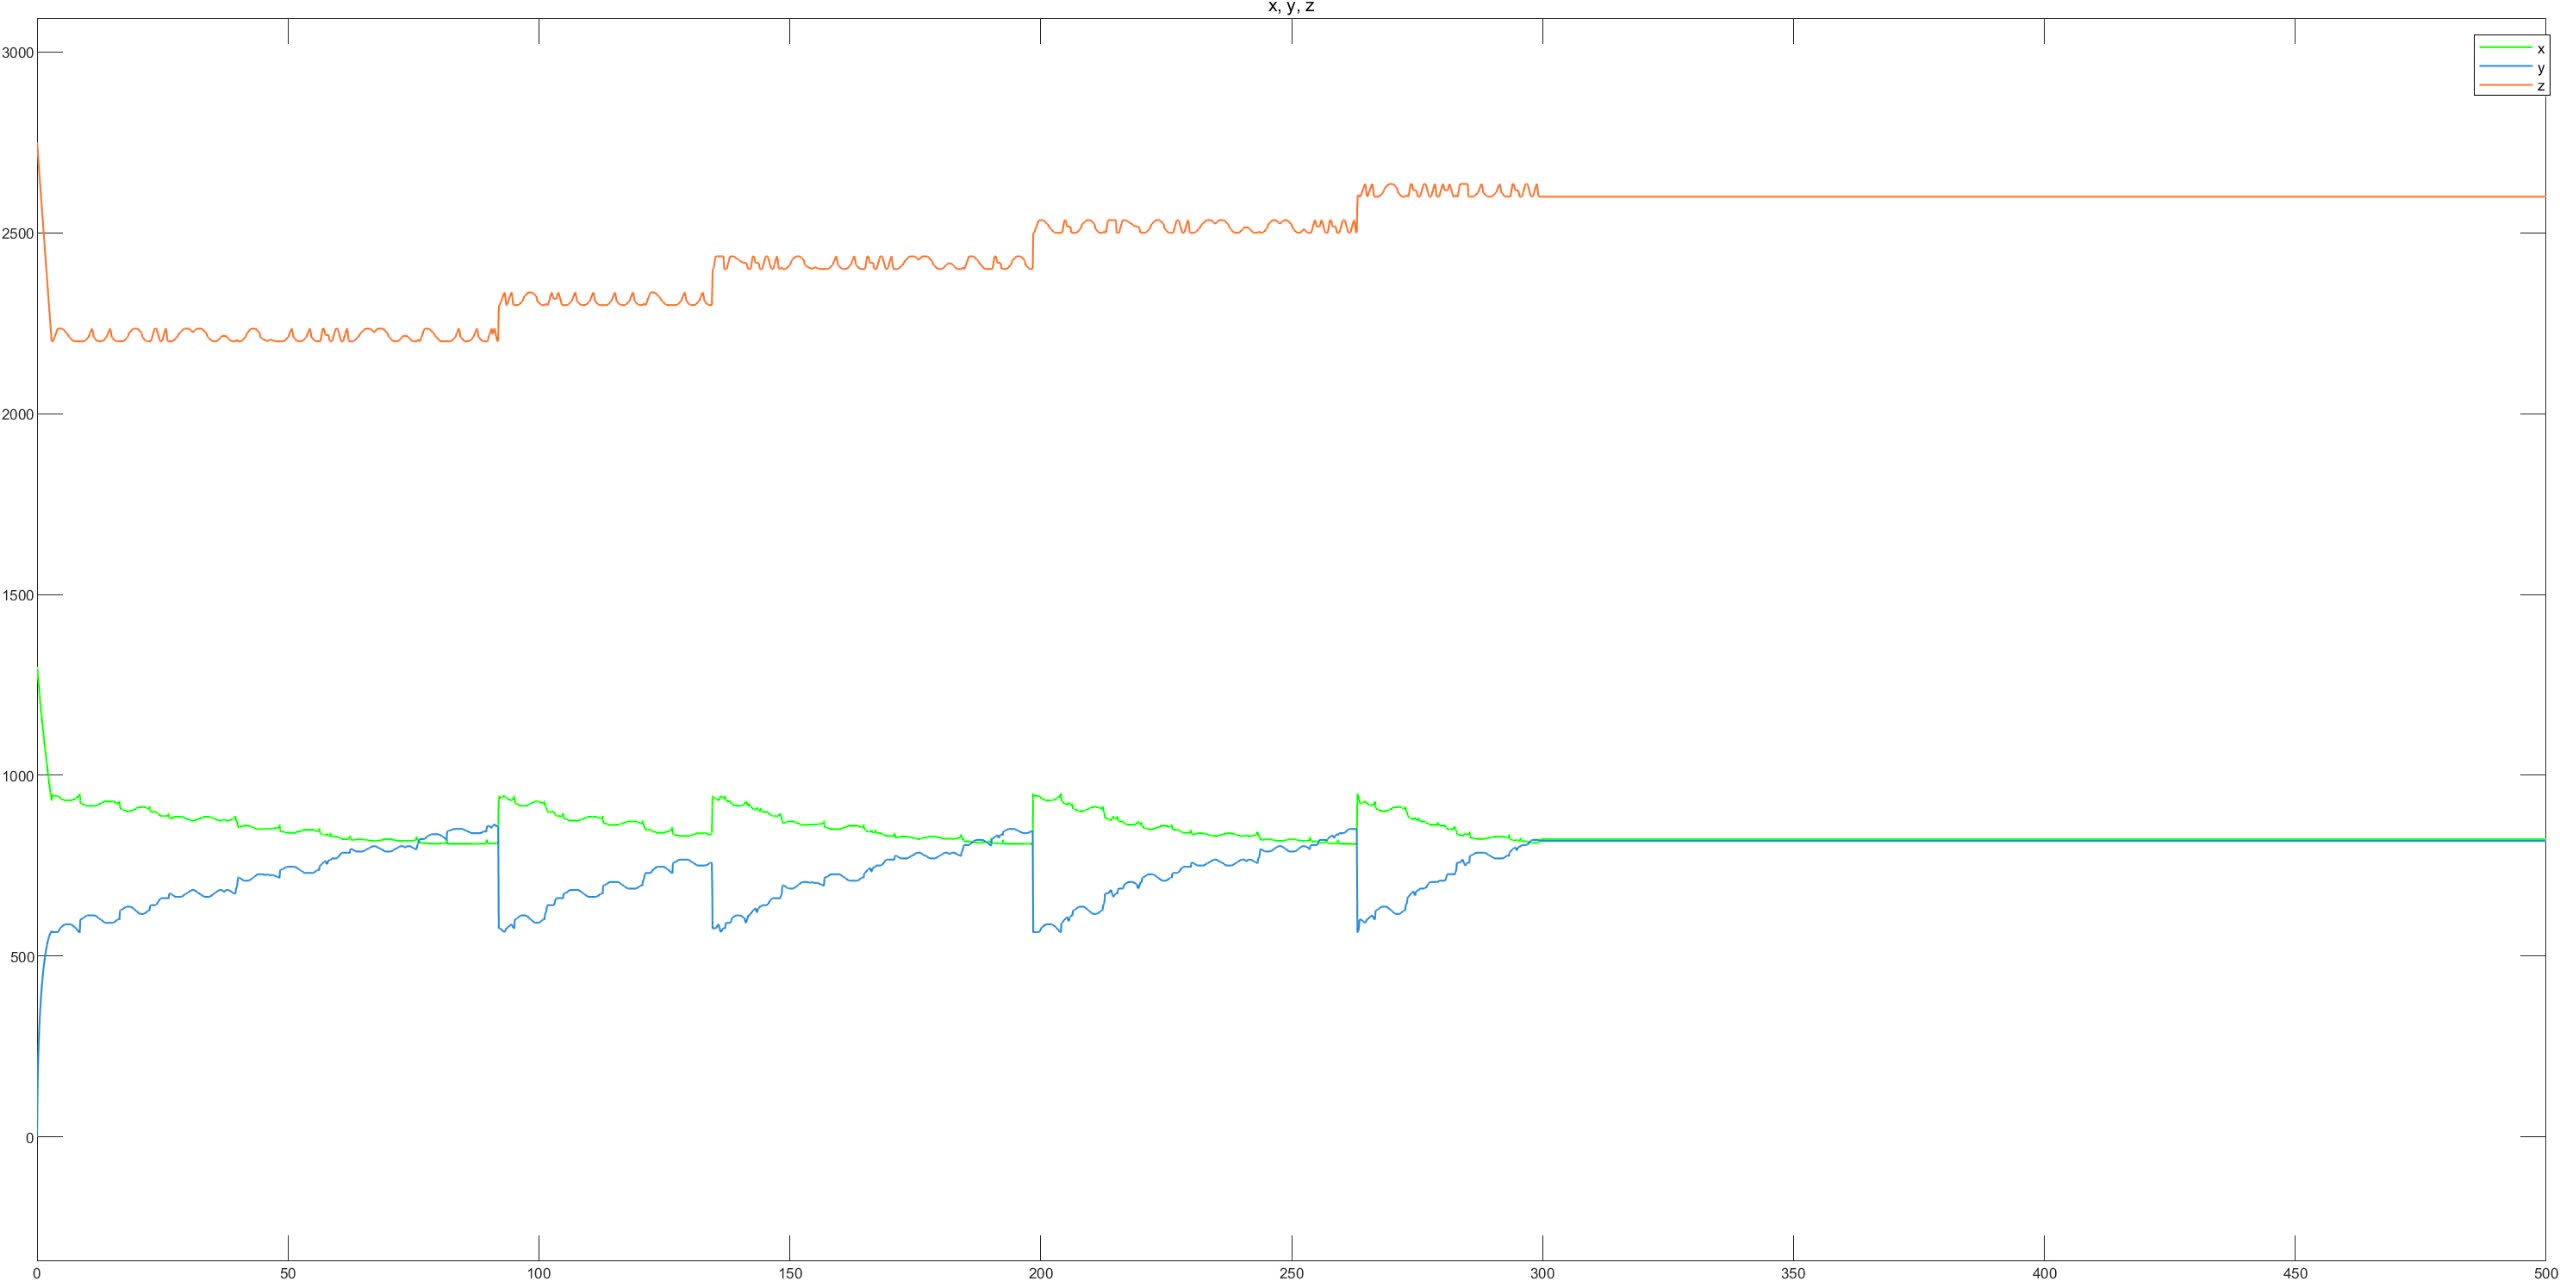
\includegraphics[width=1\textwidth]{pictures/xyz_pos_sensor.png}
        \caption{Position of robot}
        \label{fig:position}
    \end{figure}
    Result on YZ plane
    \begin{figure}[H]
        \centering
        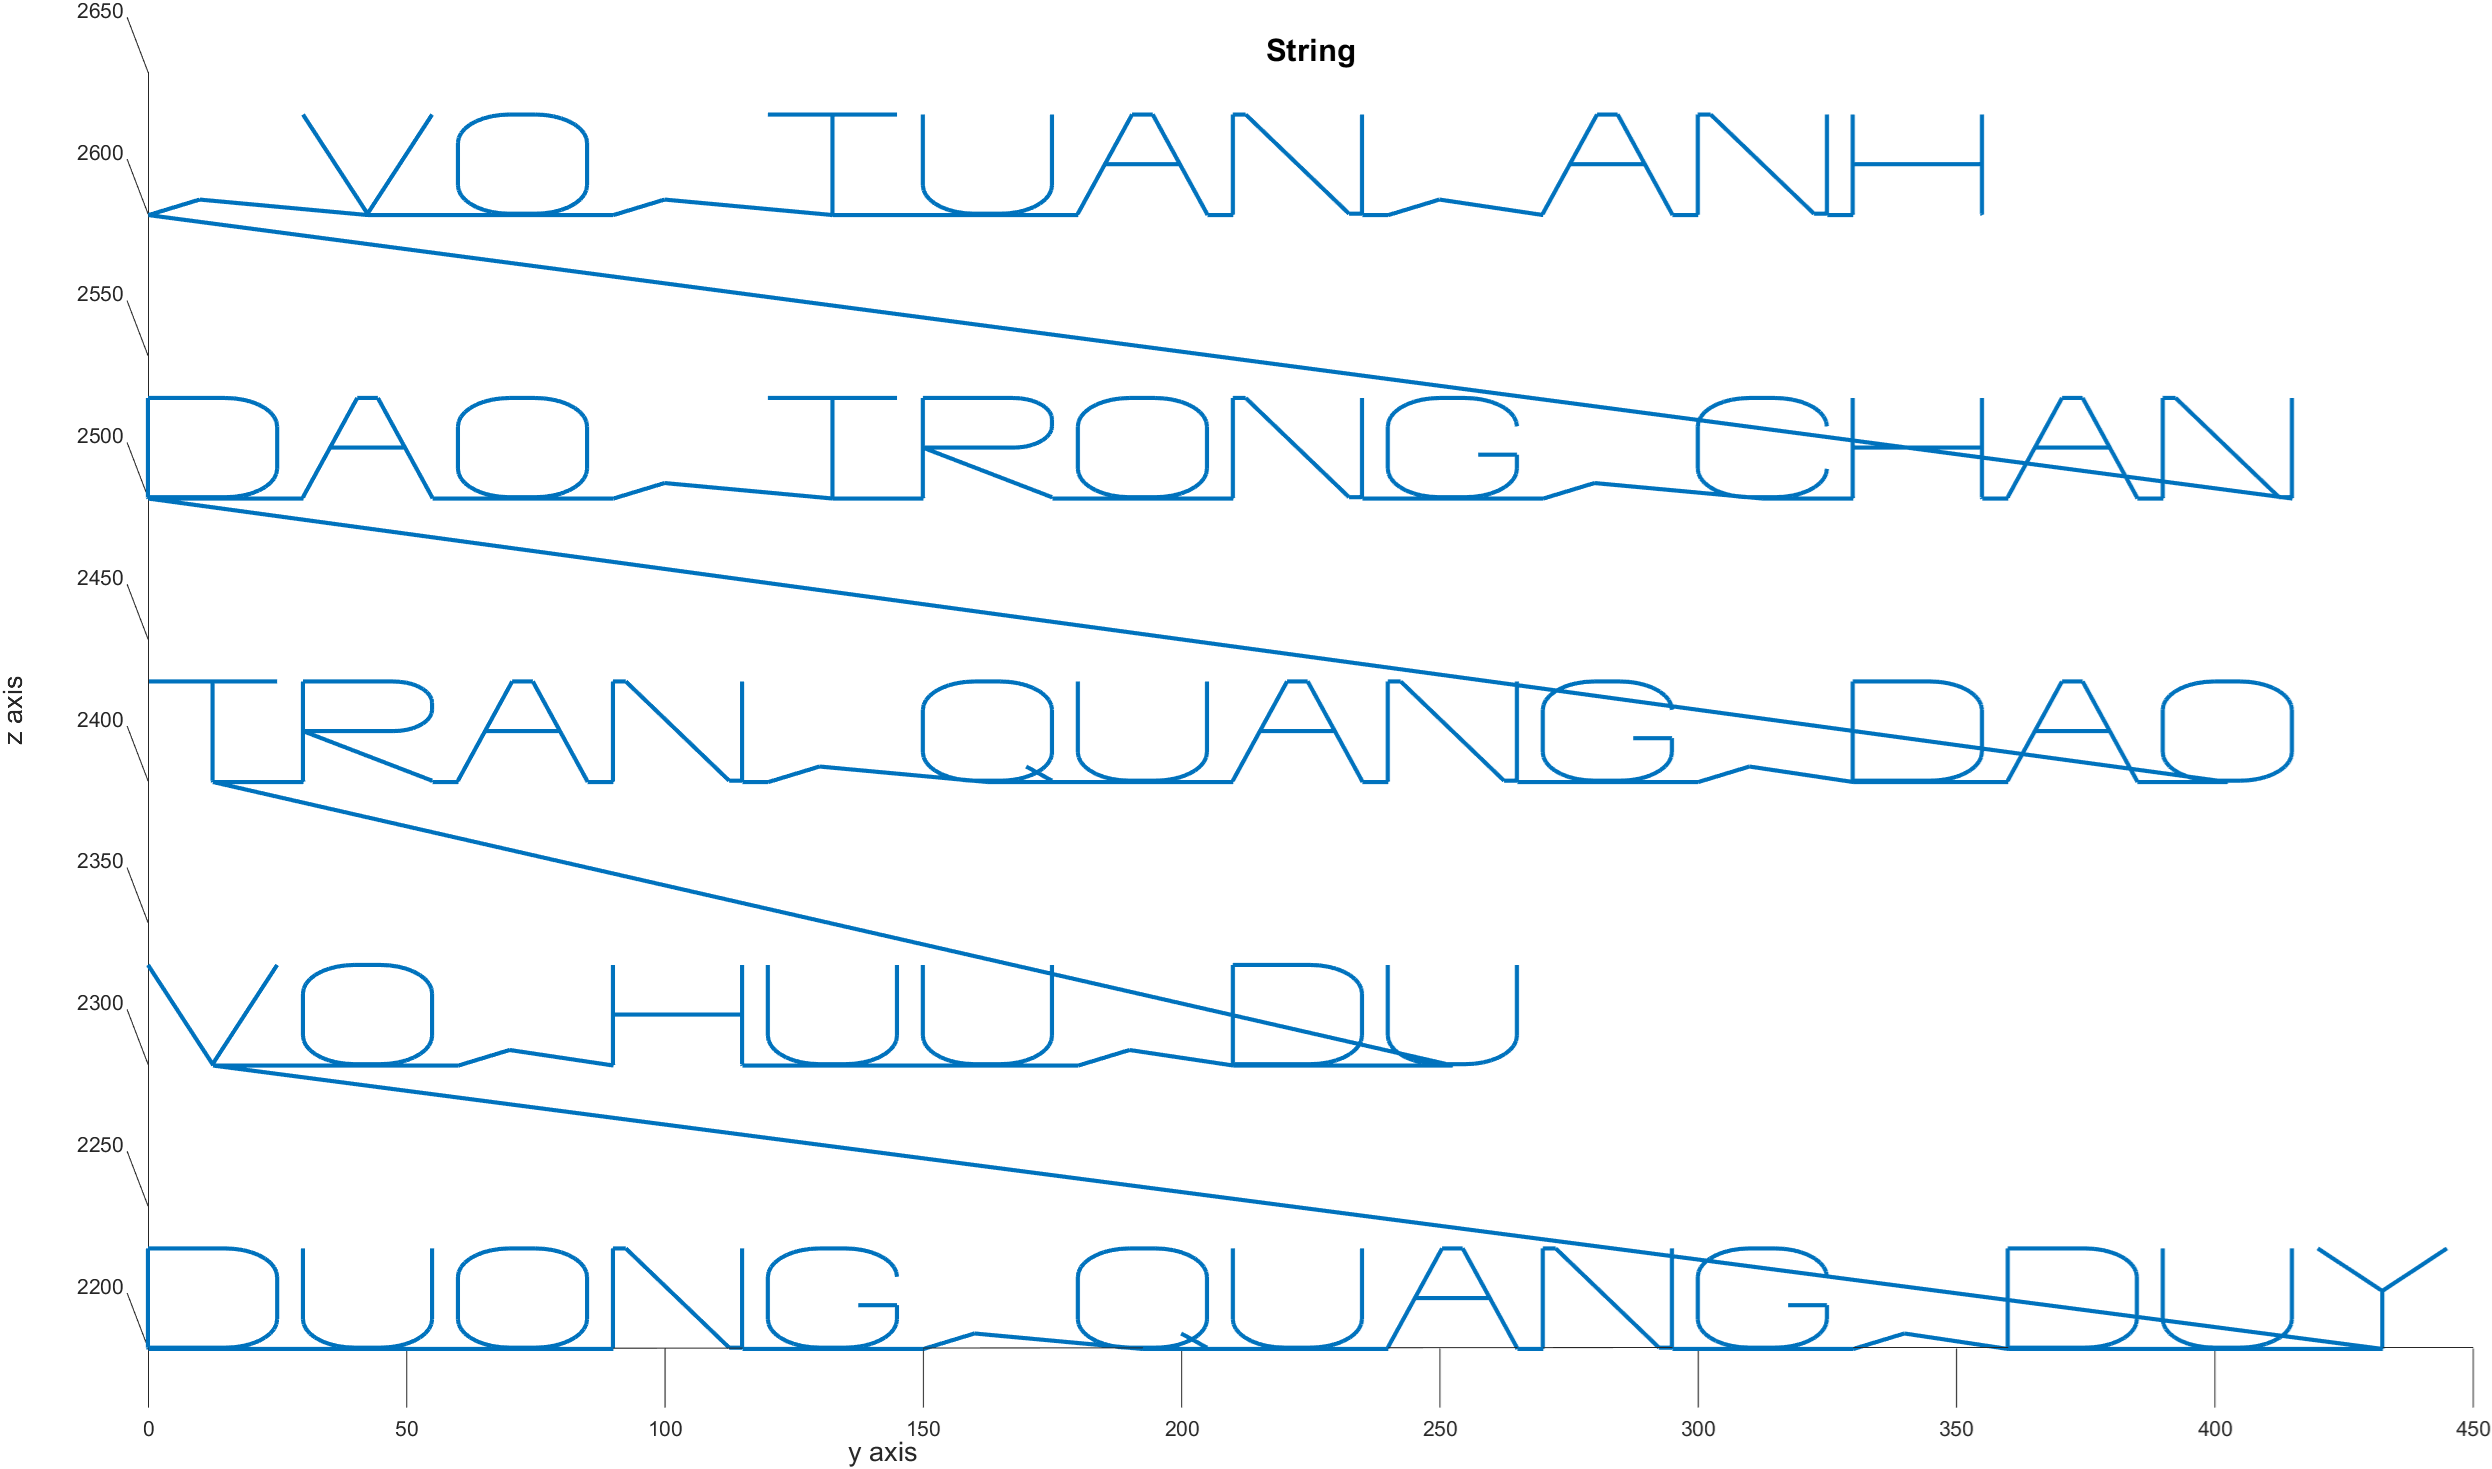
\includegraphics[width=0.8\textwidth]{pictures/result_yz.png}
        \caption{Result on YZ plane}
        \label{fig:yz_plane}
    \end{figure}
    \chapter{RESULTS}
\href{https://www.youtube.com/watch?v=eX1qE90ZBqs}{Kết quả mô phỏng được đăng trên Youtube tại đây}
    % \makeatletter
    % \renewcommand{\appendixname}{Phụ lục}         % Dùng cho tiêu đề trong trang chương
    % \renewcommand{\appendixtocname}{Phụ lục}       % Dùng cho tiêu đề trong Mục lục
    % \renewcommand{\@chapapp}{Phụ lục}              % Dùng cho 'Phụ lục A', 'Phụ lục B'
    % \makeatother
    % \begin{appendices}
    %     % \chapter{Code Matlab và Simulink}
    \section{Sơ đồ hệ thống điều khiển}
    \begin{figure}[H]
        \centering
        \includegraphics[width=1\textwidth]{pictures/ctc.png}
        \caption{Sơ đồ chung hệ thống điều khiển CTC}
    \end{figure}

    \section{Khối Dynamics}
    \begin{figure}[H]
        \centering
        \includegraphics[width=1\textwidth]{pictures/dynamic_ctc.png}
    \end{figure}
    \begin{lstlisting}[caption={Code khối Dynamic Block}, label={lst:pz}]
        function dd_state = fcn(torque, state, d_state)
            % Define constant
            g = 9.81;
            r = 0.077;
            Mw = 0.3;
            Mp = 6;
            Iw = 0.0017;
            Ip = 0.29;
            l = 0.2;
            km = 0.0458;
            ke = 0.0458;
            R = 2.49;
        
        
            % Define variables
            x = state(1);
            theta = state(2);
            dx = d_state(1);
            dtheta = d_state(2);
    
            % Compute dynamic matrix
            M = ... 
            [Mp + 2*Mw + (2*Iw)/r^2, Mp*l*cos(theta);
                Mp*l*cos(theta),     Mp*l^2 + Ip];
            
            C =... 
            [0, -Mp*dtheta*l*sin(theta);
            0,                       0];
            
            V =... 
            [-Mp*dtheta^2*l*sin(theta);
                                    0];
            
            G = ...
            [                 0;
            -Mp*g*l*sin(theta)];
            
            B = [2/r; -2];
            
            % Compute acceleration
            dd_state = inv(M)*(torque - G - V); 
    \end{lstlisting}


    \section{Khối Computed-Torque Control + Input}
    \begin{figure}[H]
        \centering
        \includegraphics[width=1\textwidth]{pictures/ref_ctc.png}
    \end{figure}
    \begin{lstlisting}[caption={Code khối Computed-Torque Control}, label={lst:step}]
        function torque = fcn(state, d_state, u, ref_ddstate)
        % Define constant
        g = 9.81;
        r = 0.077;
        Mw = 0.3;
        Mp = 6;
        Iw = 0.0017;
        Ip = 0.29;
        l = 0.2;
        km = 0.0458;
        ke = 0.0458;
        R = 2.49;     
        
        % Define variables
        x = state(1);
        theta = state(2);
        dx = d_state(1);
        dtheta = d_state(2);
               
        M = ... 
        [Mp + 2*Mw + (2*Iw)/r^2, Mp*l*cos(theta);
               Mp*l*cos(theta),     Mp*l^2 + Ip];        
         
        C =... 
        [0, -Mp*dtheta*l*sin(theta);
        0,                       0];
         
         
        V =... 
        [-Mp*dtheta^2*l*sin(theta);
                                0];
         
         
        G = ...
        [                 0;
        -Mp*g*l*sin(theta)];
        
        
        
        B = [2/r; -2];
        B_dagger = pinv(B); 
        
        %tau is scalar
        tau = B_dagger * (M *(ref_ddstate - u) + V + G);

        
        torque = (M*(ref_ddstate - u) + V + G);       
    \end{lstlisting}



    

    % \end{appendices}
    \nocite{*}
        \printbibliography[heading=bibintoc]
    
\end{document}